\chapter{Cost Model Spreadsheets}\label{app:B_cost_model_spreadsheets}

\section{Static NPV Model}\label{app:B_static_model}
The static model described in Section \ref{ch4:cm_concept} was implemented in Microsoft Excel as a single worksheet for cost analysis. Figures \ref{fig:static_model_sheet1} and \ref{fig:static_model_sheet2} show the model when flow rate is pre-defined and capacity depends on the input temperature of the produced brine. Not shown is the supporting look-up table for the EIA STEO-based electricity price forecast (Figure \ref{fig:electricity_pricing}).
%\vfill
%\pagebreak

\begin{figure}[H]
\centering
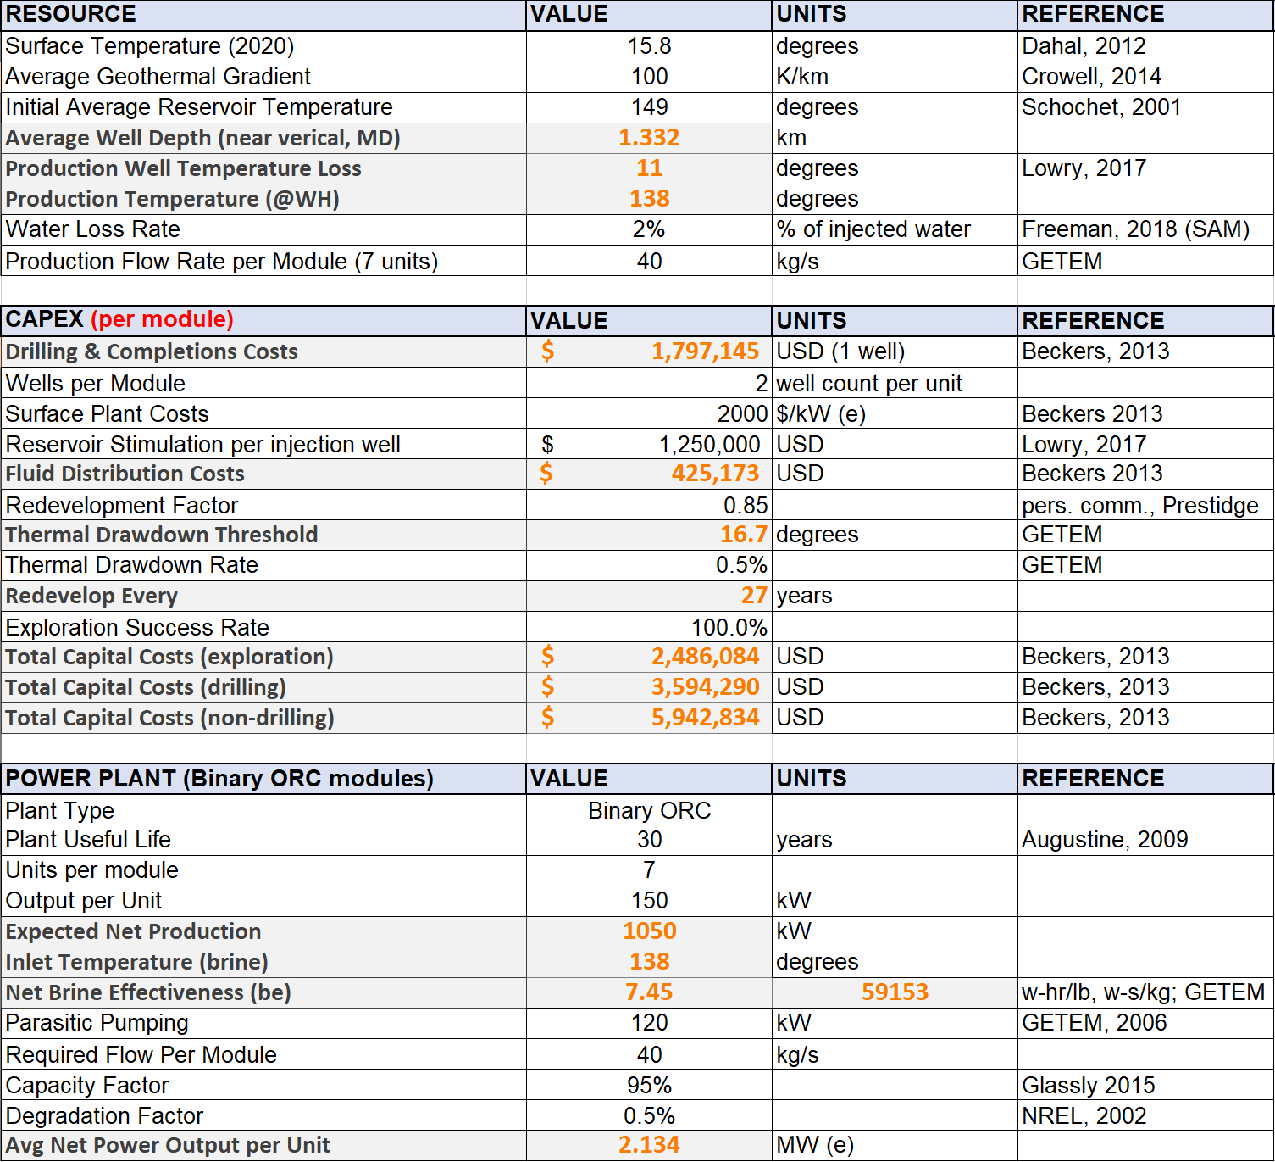
\includegraphics[width=\textwidth]{templates/images/Figure-Static_Model_SheetA.pdf}
\caption[Static cost model spreadsheet (part 1)]{First part of static NPV cost model spreadsheet for the geothermal expansion project. Values in gray cells with orange font are calculated using inputs from the rest of the sheet.}
\label{fig:static_model_sheet1}
\end{figure}

\begin{figure}[H]
\centering
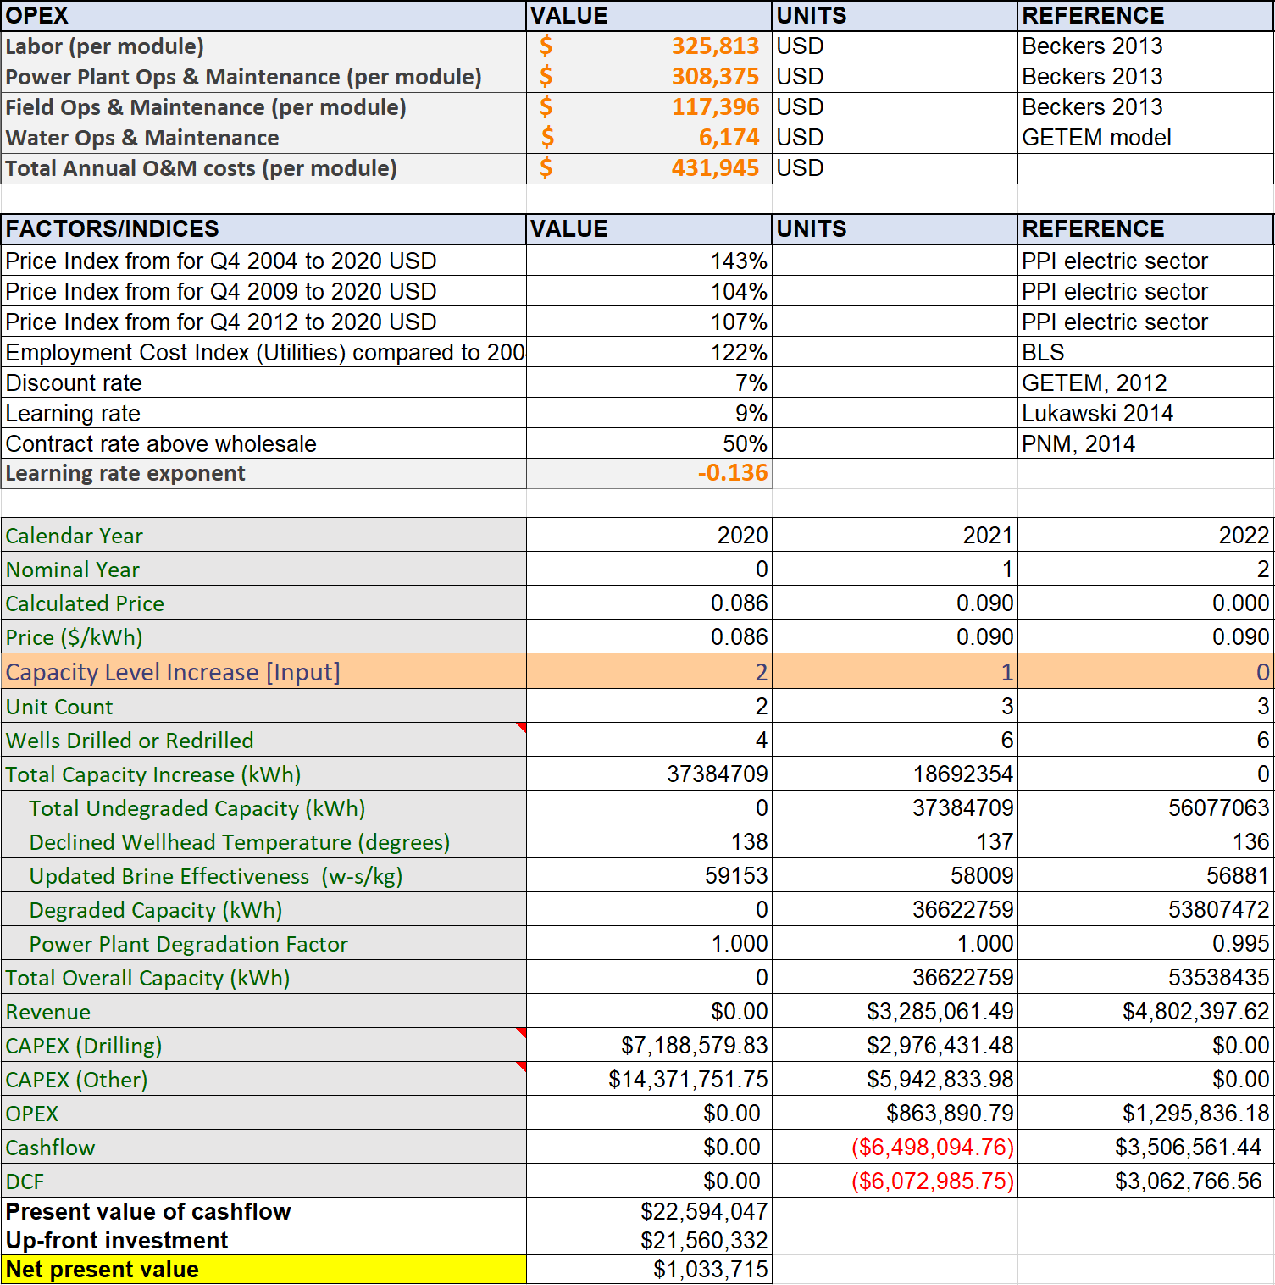
\includegraphics[width=\textwidth]{templates/images/Figure-Static_Model_SheetB.pdf}
\caption[Static cost model spreadsheet (part 2)]{Second part of static NPV cost model spreadsheet for the geothermal expansion project. Parameters in gray cells with orange font are calculated using inputs from the rest of the sheet. The orange cells in the annual cash flow analysis are manual entry fields for constructing power-plant modules. The analysis only extends out to year 2 for visualization purposes, but continues to year 30 in the complete spreadsheet.}
\label{fig:static_model_sheet2}
\end{figure}

%\pagebreak
\section{Probabilistic NPV Models}\label{app:B_flex_models}
The probabilistic NPV model was implemented as an extension of the static NPV model in Excel, with variable look-ups using the PDFs described in Section \ref{ch4:pdfs}. Flexible design options described in Section \ref{ch4:flex_design_options} were implemented as decision rules in the cash flow analysis. Figures \ref{fig:probabilistic_model_sheet1} and \ref{fig:probabilistic_model_sheet2} illustrate the spreadsheet for the Full Flexibility case (see Section \ref{ch4:flex_reduce_case}). The results histogram, target curve, and summary statistics were generated using a 2000-row data table tied to the NPV calculation cell (not shown).
%\vfill
%\pagebreak

\begin{figure}[H]
\centering
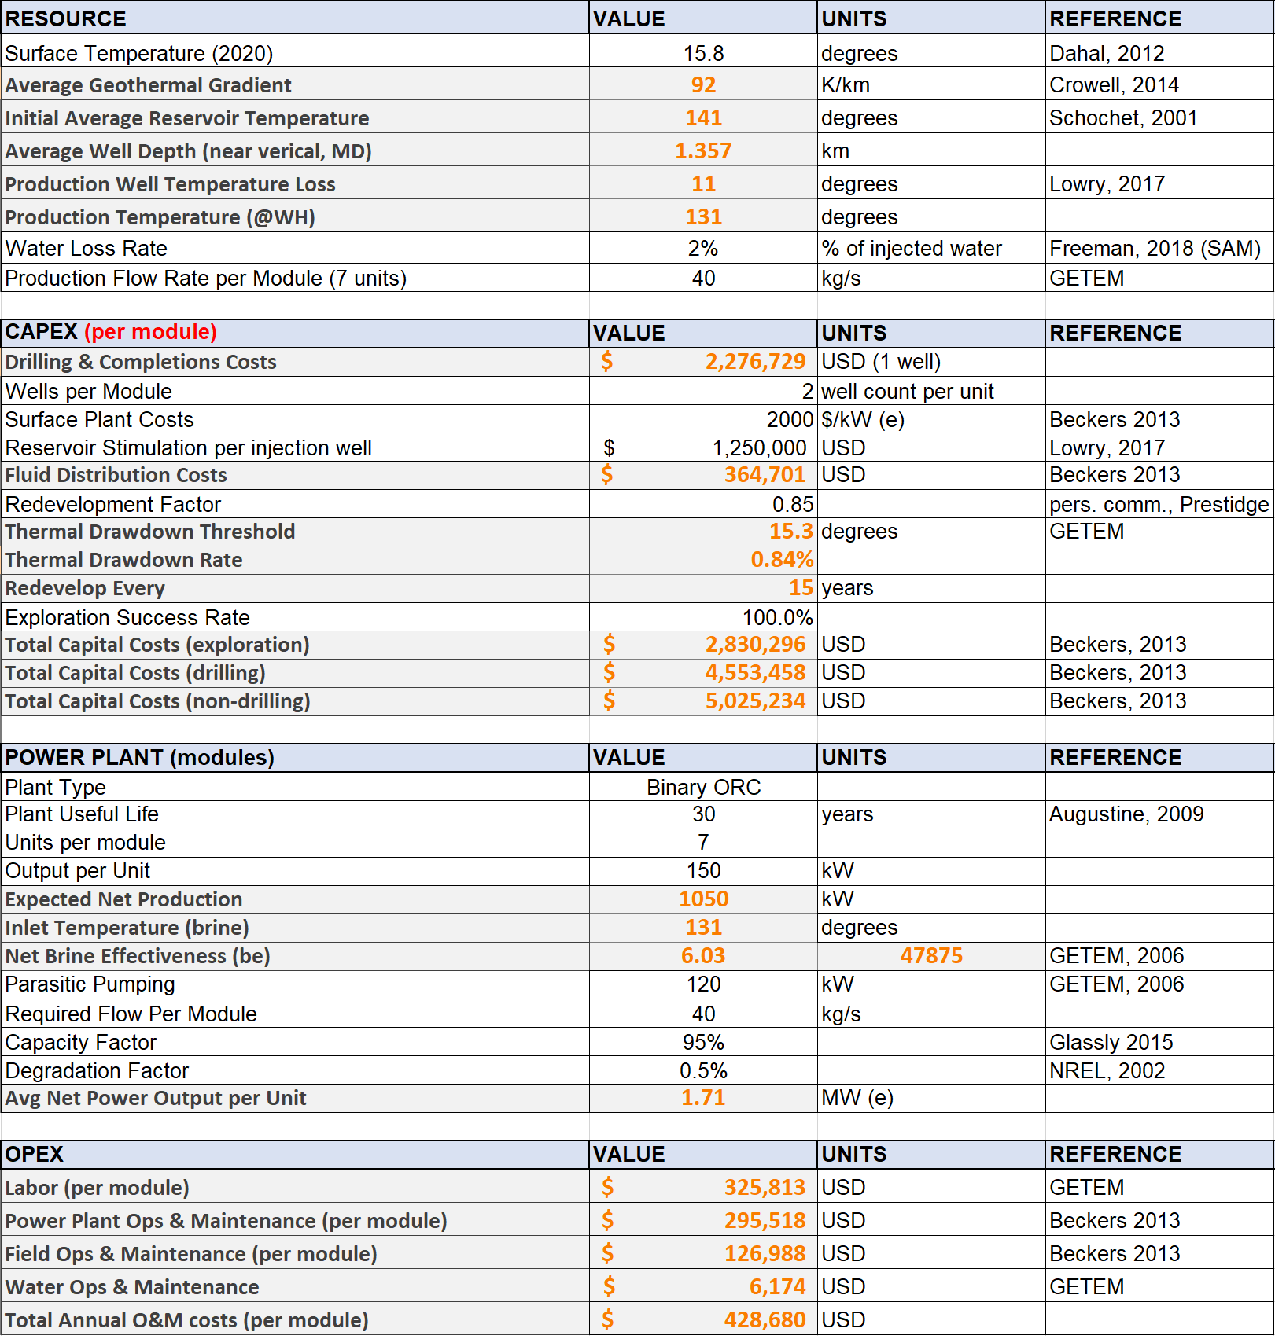
\includegraphics[width=\textwidth]{templates/images/Figure-Flexible_Model_SheetA.pdf}
\caption[Probabilistic cost model spreadsheet (part 1)]{First part of probabilistic NPV cost model spreadsheet for the geothermal expansion project. Values in gray cells with orange font are calculated using inputs from the sheet or distributions in other worksheets. PDF look-ups are implemented for Average Geothermal Gradient, Initial Average Reservoir Temperature, Drilling \& Completions Costs, Thermal Drawdown Rate, and Price Forecast.}
\label{fig:probabilistic_model_sheet1}
\end{figure}

\begin{figure}[H]
\centering
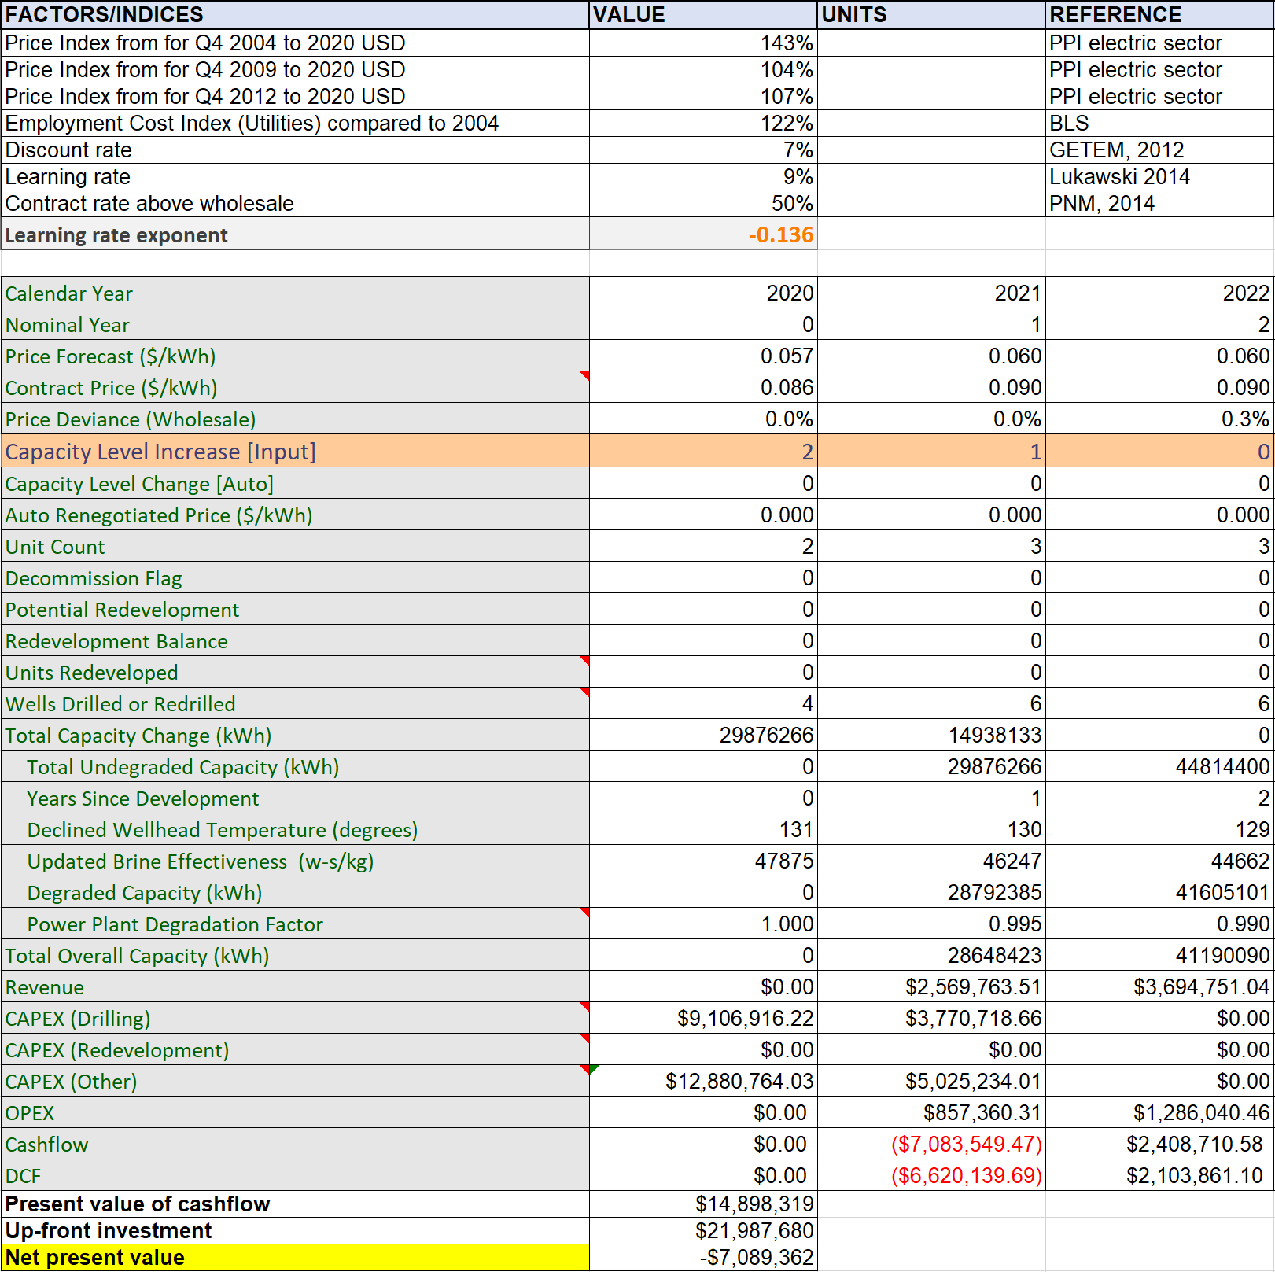
\includegraphics[width=\textwidth]{templates/images/Figure-Flexible_Model_SheetB.pdf}
\caption[Probabilistic cost model spreadsheet (part 2)]{Second part of probabilistic NPV cost model spreadsheet for the geothermal expansion project. Parameters in gray cells with orange font are calculated using inputs from the rest of the sheet. PDF look-ups are implemented for Average Geothermal Gradient, Initial Average Reservoir Temperature, Drilling \& Completions Costs, Thermal Drawdown Rate, and Price Forecast. The orange cells in the annual cash flow analysis are manual entry fields for constructing power-plant modules. Decision rules are implemented in the annual cash flow section. The yearly breakdown of cost and revenue only extends out to year 2 for visualization purposes, but continues to year 30 in the full spreadsheet.}
\label{fig:probabilistic_model_sheet2}
\end{figure}